\documentclass[12pt]{article}
% \usepackage[brazilian]{babel}
\usepackage[a4paper,inner=3cm,outer=3cm, total={6in, 8in}]{geometry}
\usepackage[utf8]{inputenc}
\usepackage{lmodern}
\usepackage{graphicx}
\usepackage{float}
\usepackage{newtxmath}
\usepackage{amssymb, amsmath, amsfonts, array}
\usepackage{bm}
\usepackage{indentfirst}

\title{TIP8419 - Tensor Algebra\\ 
       Homework 0}
\author{Ezequias Márcio - $497779$}
\date{\today}

\begin{document}

\maketitle

\section*{Hadamard, Kronecker and Khatri-Rao Products}\vspace{.5cm}

\textbf{Problem 1.} For randomly generated matrices $\bm{A}$ and $\bm{B}\in 
\mathbb{C}^{N\times N}$, create an algorithm to compute the Hadamard Product 
$\bm{A} \odot \bm{B}$. Then, compare the run time of your algorithm with
the operator \texttt{.$\ast$} of the software Octave/Matlab\textregistered. 
Plot the run time curve as a function of the number of rows/columns 
$N \in \{2,4,8,16,32,64,128\}$.\\

\noindent \textbf{Solution:}
%------------------------------------------------------------------------------
The proposed algorithm to calculate the Hadamard product was implemented in 
\texttt{python} and the code listing can be found in the file 
\texttt{tensoralg.py}. 

In Figure \ref{hadm}, we can see the the difference of 
execution time between the proposed algorithm and the native Numpy function. As much as $N$ increases, the Numpy function \texttt{.$\ast$} 
presented the best performance.\\

\begin{figure}[!ht]
    \centering 
    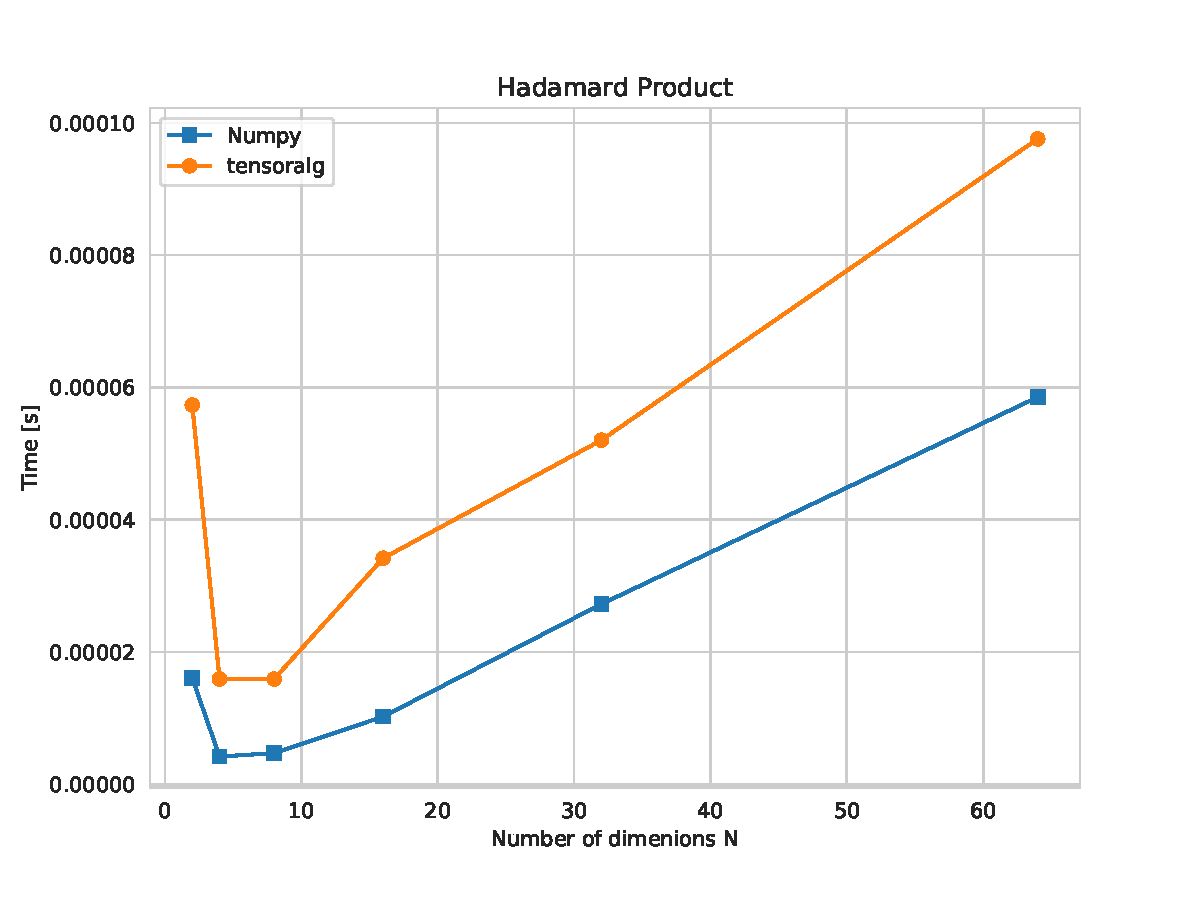
\includegraphics[width=0.55\linewidth]{figs/hadm.pdf}
    \caption{Comparsion of Hadamard product implementations.}
    \label{hadm}
\end{figure}
%------------------------------------------------------------------------------

\noindent
\textbf{Problem 2.} For randomly generated matrices $\bm{A}$ and $\bm{B}\in 
\mathbb{C}^{N\times N}$, create an algorithm to compute the Kronecker Product 
$\bm{A} \otimes \bm{B}$. Then, compare the run time of your algorithm with
the operator \texttt{kron($\bm{A}, \bm{B}$)} of the software 
Octave/Matlab\textregistered. Plot the run time curve as a function of the 
number of rows/columns $N \in \{2,4,8,16,32,64,128\}$.\\

\noindent \textbf{Solution:}
%------------------------------------------------------------------------------
% Numpy broadcasting match the dimensions and the condition row major reshape...
The proposed algorithm to calculate the Kronecker product also was implemented 
in \texttt{python} and the code listing can be found in the file 
\texttt{tensoralg.py}. In Figure \ref{kron}, we can see the the difference of 
between the two algorithms.

As much as $N$ increases, the Numpy function \texttt{np.kron} is outperformed 
by the tensoralg implementation with respect to the case that are considering 
only two matrices.\\

\begin{figure}[!ht]
       \centering 
       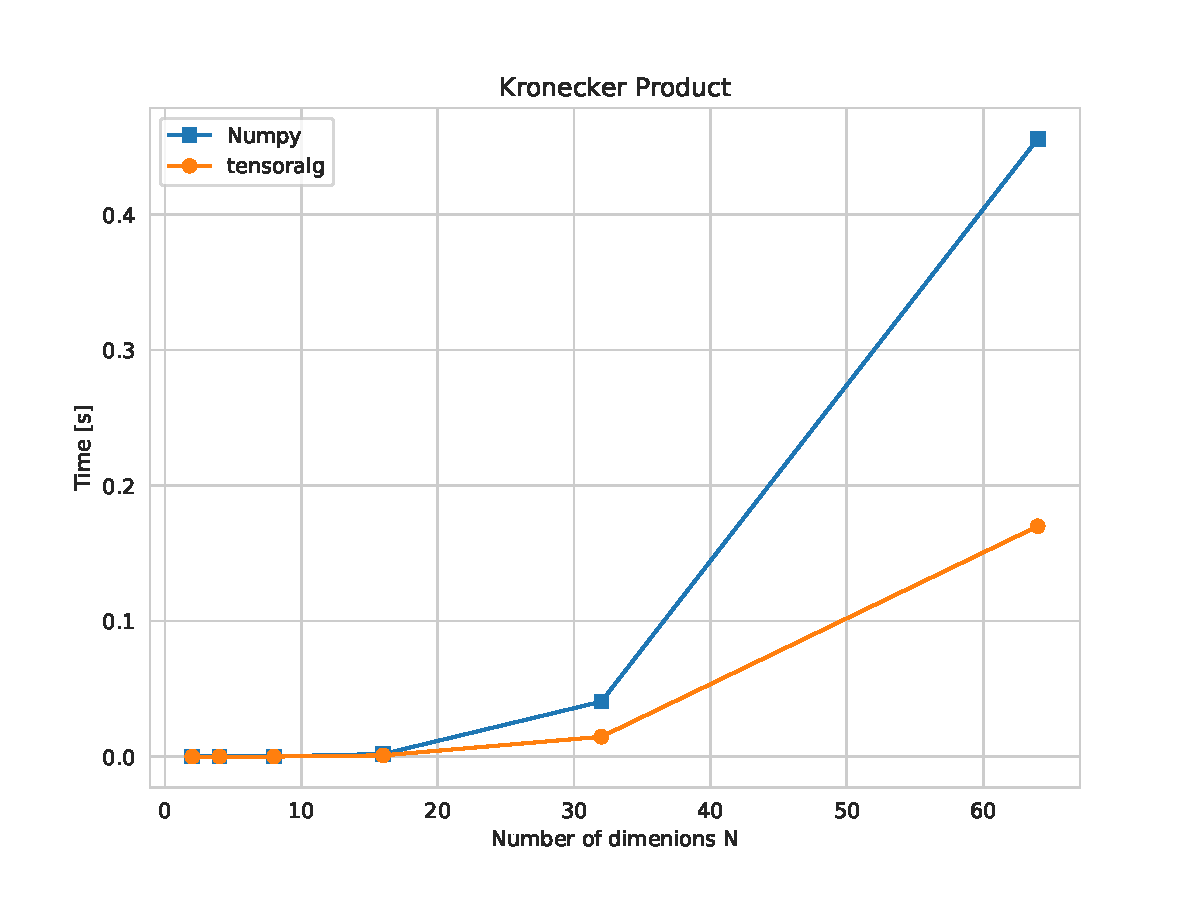
\includegraphics[width=0.55\linewidth]{figs/kron.pdf}
       \caption{Comparsion of Kronecker product implementations.}
       \label{kron}
   \end{figure}
%------------------------------------------------------------------------------

\noindent
\textbf{Problem 3.} For randomly generated matrices $\bm{A}$ and $\bm{B}\in 
\mathbb{C}^{N\times N}$, create an algorithm to compute the Khatri-Rao Product 
$\bm{A} \diamond \bm{B}$ according with the following prototype function:
\begin{equation*}
\bm{R} = \mathit{kr}(\bm{A}, \bm{B})    
\end{equation*}

\noindent \textbf{Solution:}
Again, the proposed algorithm to calculate the Khatri-Rao product was 
implemented in \texttt{python} and the code listing can be found in the file 
\texttt{tensoralg.py}

Additionally, the comparsion between the proposed algorithm...

%------------------------------------------------------------------------------
\begin{figure}[!ht]
       \centering 
       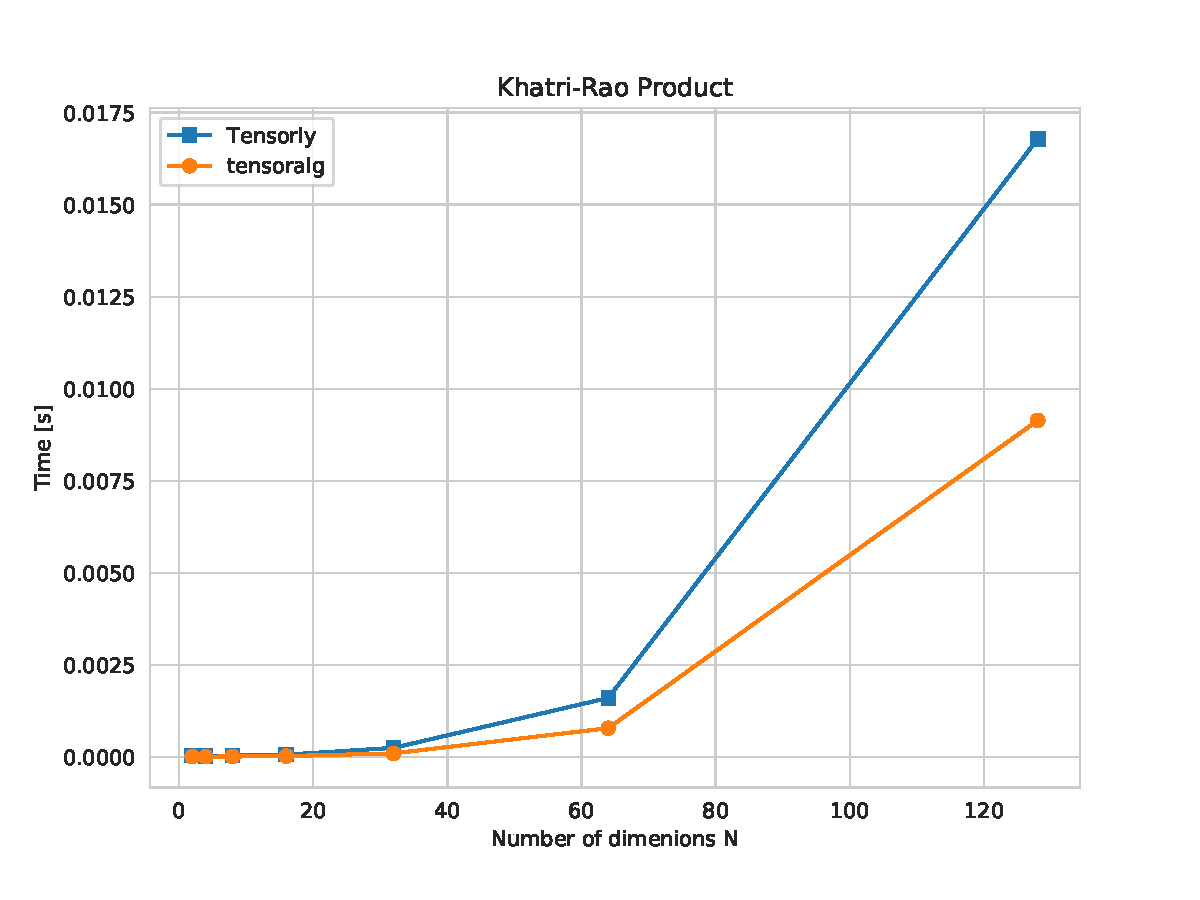
\includegraphics[width=0.55\linewidth]{figs/krao.pdf}
       \caption{Comparsion of Khatri-Rao product implementations.}
       \label{krao}
   \end{figure}
%------------------------------------------------------------------------------


\end{document}
